\documentclass[a4paper, 14pt]{extarticle}
\usepackage[russian]{babel}
\usepackage[T1]{fontenc}
\usepackage{fontspec}
\usepackage{indentfirst}
\usepackage{enumitem}
\usepackage{graphicx}
\usepackage[
  left=20mm,
  right=10mm,
  top=20mm,
  bottom=20mm
]{geometry}
\usepackage{parskip}
\usepackage{titlesec}
\usepackage{xurl}
\usepackage{hyperref}
\usepackage{float}
\usepackage[
  figurename=Рисунок,
  labelsep=endash,
]{caption}
\usepackage[outputdir=build, newfloat]{minted}

\hypersetup{
  colorlinks=true,
  linkcolor=black,
  filecolor=blue,
  urlcolor=blue,
}

\renewcommand*{\labelitemi}{---}
\setmainfont{Times New Roman}
\setmonofont{JetBrains Mono}[
  SizeFeatures={Size=11},
]

\newenvironment{code}{\captionsetup{type=listing}}{}
\SetupFloatingEnvironment{listing}{name=Листинг}

\setminted{
  fontsize=\footnotesize,
  frame=lines,
  framesep=2mm,
}

\setlength{\parskip}{6pt}

\setlength{\parindent}{1cm}
\setlist[itemize]{itemsep=0em,topsep=0em,parsep=0em,partopsep=0em,leftmargin=2.0cm,wide}
\setlist[enumerate]{itemsep=0em,topsep=0em,parsep=0em,partopsep=0em,leftmargin=2.0cm,wide}

\renewcommand{\thesection}{\arabic{section}.}
\renewcommand{\thesubsection}{\thesection\arabic{subsection}.}
\renewcommand{\thesubsubsection}{\thesubsection\arabic{subsubsection}.}

\titleformat{\section}{\normalfont\bfseries}{\thesection}{0.5em}{}
\titleformat{\subsection}{\normalfont\bfseries}{\thesubsection}{0.5em}{}

\titleformat*{\section}{\normalfont\bfseries}
\titleformat*{\subsection}{\normalfont\bfseries}

\linespread{1.5}
\renewcommand{\baselinestretch}{1.5}

\begin{document}

\begin{titlepage}
  \vspace{0pt plus2fill}
  \noindent

  \vspace{0pt plus6fill}
  \begin{center}
    Санкт-Петербургский национальный исследовательский университет
    информационных технологий, механики и оптики

    \vspace{0pt plus3fill}

    Факультет инфокоммуникационных технологий

    Направление подготовки 11.03.02

    \vspace{0pt plus2fill}

    Лабораторная работа №7

    <<Установка Django. Создание и структура проекта. \\ Начало работы с проектом в IDE PyCharm >>

  \end{center}

  \vspace{0pt plus9fill}
  \begin{flushright}
    Выполнил: \\
    Швалов Даниил Андреевич

    Группа: К33211

    Проверила: \\
    Марченко Елена Вадимовна
  \end{flushright}

  \vspace{0pt plus2fill}
  \begin{center}
    Санкт-Петербург

    2023
  \end{center}
\end{titlepage}

\section{Введение}

\textbf{Цель работы}: научиться создавать и работать с проектами Django с
помощью виртуальных окружений Python.

\section{Ход работы}

С помощью команды \texttt{python3 -m venv tutorial-env} была создана среда
окружения. В результате выполнения команды в корневой директории появилась новая
директория tutorial-env, которая содержит в себе различные исполняемые файлы,
используемые Python. Виртуальное окружение в Python используется для того, чтобы
создавать изолированную среду. Это удобно при использовании одних и тех же
зависимостей разных версий в разных проектах.

С помощью команды \texttt{source tutorial-env/bin/activate} была активирована
виртуальная среда. Это команда прописывает все нужные пути до виртуального
окружения. Таким образом, теперь используется не системный Python, а тот, что
находится в виртуальном окружении.

С помощью команды \texttt{pip install django} был установлен фреймворк Django.
Для того, чтобы удостовериться в успешной установке фреймворка, была выполнена
команда \texttt{pip freeze}. Результат ее выполнения показан на рис.
\ref{fig:pip-freeze}.

\begin{figure}[H]
  \centering
  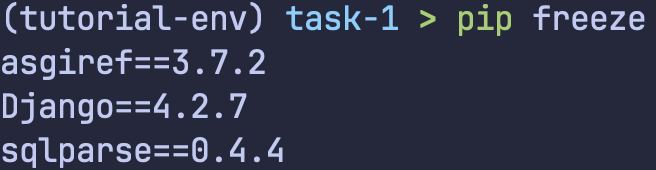
\includegraphics[width=0.6\textwidth]{images/pip-freeze.png}
  \caption{Установленные библиотеки в виртуальном окружении}
  \label{fig:pip-freeze}
\end{figure}

Для создания проекта Django использовалась команда \texttt{django-admin
  startproject blogfspo}. После ее выполнения в корневой директории появилась
новая директория blogfspo, содержащая файлы проекта. Утилита
\texttt{django-admin} используется для создания и управления проектами Django.
Внутри директории blogfspo находится директория с таким же названием. Файлы,
находящиеся в ней, используются для настройки проекта.

Каждый проект Django состоит из приложений. Каждое такое приложение представляет
собой некую изолированную часть функциональности, которая имеет полностью
самостоятельный программный код (система авторизации, система оплаты и т.п.).
Эти приложения могут переноситься в любые другие приложения. Для создания нового
приложения blog использовалась команда \texttt{python manage.py startapp blog}.
На рис. \ref{fig:pycharm} показана структура получившегося проекта.

\begin{figure}[H]
  \centering
  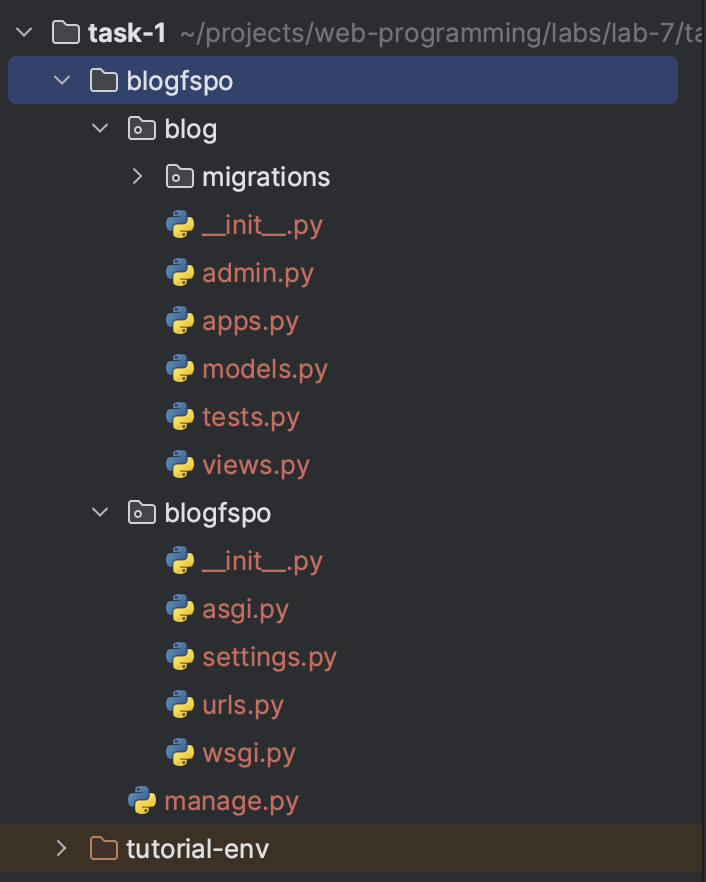
\includegraphics[width=0.5\textwidth]{images/pycharm.png}
  \caption{Структура проекта}
  \label{fig:pycharm}
\end{figure}

Команда \texttt{python manage.py} используется для тех же задач, что и утилита
\texttt{django-admin}. Единственное отличие в том, что \texttt{manage.py}
устанавливает переменную окружения \texttt{DJANGO\_SETTINGS\_MODULE}, которая
указывает на файл \texttt{settings.py} в проекте. Это позволяет применять
настройки именно к данному проекту.

\section{Вывод}

В ходе выполнения лабораторной работы я научился создавать и работать с
проектами Django с помощью виртуальных окружений Python.

\end{document}
